\section{Präparation und Charakterisierung der Substrate für 2DES auf Heliumfilmen}

\subsection{Anforderungen an die Substrate}

Im Folgenden sind die experimentellen Anforderungen an Substrate für 2DES auf dünnen Heliumfilmen zusammengefasst:
\begin{description}
	\item[Oberflächenrauigkeit:] Da die Größenordnungen im System durch die üblichen Filmdicken und den Abstand der Elektronen untereinander vorgegeben sind, sollte die Oberflächenrauigkeit des verwendeten Substrates im Vergleich dazu deutlich geringere typische Längen besitzen.
	\item[Isolierschicht:] Bisher war eine isolierende Schicht auf der Substratoberfläche unbedingt notwendig, um höhere Elektronendichten erreichen zu können. Allerdings gibt es Hinweise darauf, dass auch Silizium"=Substrate nur mit der natürlichen Oxidschicht als Unterlage für ein 2DES verwendet werden können. Das Erreichen von sehr hohen Elektronendichten wegen des bei Filmdicken unter \unit[3.5]{nm} auch bei sehr glatten Substraten auftretenden Tunnelns von Elektronen wird jedoch erschwert sein.
	\item[Laterale Abmessungen:] Eine Möglichkeit, eine Verschmierung der Phasenübergänge gering zu halten, ist die Reduzierung der effektiven Substratfläche. Die Konstanz der Amplitude des elektrischen Hochfrequenzfeldes wird über eine kleinere Probenfläche hinweg besser sein. Ein begrenzender Faktor ist hierbei das mit der geringeren Anzahl von an der Messung beteiligten Elektronen verbundene Zurückgehen des Signal"=Rausch"=Abstands der gemessenen Parameter. 
	\item[Schwache Leitfähigkeit:]
Speziell für das Experimentieren mit 2DES in einem Mikrowellen"=\HR\ muss man die elektrischen Eigenschaften des Substrats berücksichtigen. Da man kein metallisches Substrat in den Resonator einbauen kann, jedoch ein Potential als Haltespannung an das Substrat anlegen möchte, blieb bisher nur die Möglichkeit undotiertes Silizium für diese Zwecke zu verwenden. Nach einigen Versuchen mit aufgedampften Kohlenstoff"=Filmen hat sich gezeigt, dass man diese ebenfalls mit für das Experiment günstigen Eigenschaften herstellen kann und noch dazu die Freiheit hat, ein beliebiges isolierendes Substratmaterial als Substrat zu verwenden. Erste Versuche wurden mit Kohlenstoff"=Filmen auf Glas durchgeführt, worauf in Abschnitt~\ref{ssec:kohlenstoff} genauer eingegangen wird; es sind jedoch auch andere Trägermaterialien für diese Filme denkbar.
\end{description}

\subsection{Überblick über verwendete Substrate}

Bisher wurden nur zugeschnittene Siliziumwafer als Trägermaterial für verschiedene isolierende Deckschichten verwendet. In der folgenden Liste sind die verwendeten Isolierschichten für die Messungen an 2DES hoher Dichte auf Heliumfilmen aufgeführt und kurz beschrieben:
\begin{description}
	\item [PMMA:] mittels Spin"=Coating auf das Silizium"=Plättchen aufgebracht. Mit diesem Substrat wurde der am besten Reproduzierbare Beladeprozess in den Beladeserien untersucht. Die Spannungswerte des Beladungsbeginns lagen immer um $\unit[-0.8]{V}$. Leider waren die erreichbaren Beweglichkeiten auf diesen Substraten nicht ausreichend um auch eine Serie von Messungen der Zyklotronresonanz an 2DES auf dünnen Helium"=Filmen durchzuführen.
	\item [SiO$_2$:] oxidierte Silizium"=Wafer mit \unit[200]{nm} dicker \SiO"=Schicht\footnote{Hergestellt von der Firma Silchem in Freiberg/Sachsen.}. Mit diesen Substraten ließen sich hervorragende Elektronenbeweglichkeiten und auch sehr hohe Elektronendichten erreichen, allerdings war auch ein Großteil von Messungen mit diesen Substraten nicht möglich, da sich beim Abkühlen des Kryostaten gezeigt hat, dass der Resonator völlig überdämpft war. Dieser Effekt ließ sich leider nicht direkt nach dem Einbau der Probe bei Raumtemperatur, sondern erst beim Abkühlen auf Temperaturen des flüssigen Heliums sehen, was deshalb zu einem erheblichen zeitlichen Aufwand bei der Suche nach funktionierenden Proben führte. Mögliche Ursachen für dieses Problem sind eine bereits vorhandene starke Beladung der isolierenden Substratoberfläche oder Verunreinigungen im Silizium bzw.\ in der Oxidschicht, die dazu führen, dass die Absorption von Mikrowellen durch das Substrat sehr groß ist.
\end{description}
Da eine besonders glatte Oberfläche und eine konstante Dicke der Isolierschicht die Grundlage für eine gute Reproduzierbarkeit der Transportmessungen an 2DES auf dünnen Heliumfilmen sind, wurden bei dem Großteil der hier vorgestellten Messungen mit PMMA oder \SiO\ bedeckte Siliziumsubstrate verwendet.

\subsection{Neue Variante: Dünne Kohlenstofffilme auf beliebigen Substraten}
\label{ssec:kohlenstoff}
Bisher wurde ausschließlich undotiertes Silizium als Substrat oder Trägermaterial verwendet. Im Rahmen dieser Arbeit wurde versucht, andere Materialien für diese Aufgabe zu finden. Die Verwendung von dünnen Kohlenstofffilmen mit einer Dicke von einigen Nanometern auf einem glatten, isolierenden Trägermaterial schien die oben genannten Voraussetzungen für Substrate zu erfüllen. Die gewünschte Leitfähigkeit lässt sich hierbei einfach durch die aufgebrachte Filmdicke einstellen. Solche Kohlenstofffilme haben den entscheidenden Vorteil, dass sie sich auf nahezu beliebigen isolierenden Substraten und falls erforderlich auch strukturiert aufbringen lassen.

\subsubsection{Voruntersuchungen der Kohlenstofffilme}
Um die Bedingungen für eine Verwendung von dünnen Kohlenstofffilmen als Elektrodenmaterial zu untersuchen, wurden diese Filme mit einer Dicke von 5 bis \unit[15]{nm} für erste Untersuchungen auf Glassubstrate aufgedampft. In ersten Messungen wurde die Variation ihrer elektrischen Eigenschaften beim Abkühlen auf tiefe Temperaturen im Bereich einiger Kelvin untersucht.

Die Kohlenstofffilme wurden in einer herkömmlichen Vakuum"=Bedampfungsanlage durch Verdampfung eines stromdurchflossenen Stäbchens aus reinem Kohlenstoff erzeugt. Hierbei hat sich gezeigt, dass ein Abstand, von mehr als \unit[20]{cm}, des zu bedampfenden Substrats von der Kohlenstoffquelle die Oberflächenqualität der erhaltenen Filme verbessert. Ein Problem bereitet die Bestimmung der Filmdicke der aufgedampften Schicht, da Kohlenstoff im Gegensatz zu Metallen eine geringe Dichte besitzt. Aus diesem Grund liefert die Bestimmung der Schichtdicke mittels der Resonanzänderung eines Schwingquarzes keine vergleichbar genauen Resultate.
\begin{figure}[h!tb]
	\plotlink{C_rrr}{\includegraphics[width=\smidwidth]{exp_substrate/C_rrr}}%
	\hfill%
	\begin{minipage}[b]{\textwidth-\tabcolsep-\smidwidth}
		\caption[Messung des Restwiderstandsverhältnisses eines Kohlenstofffilms]{Messung des Widerstandes eines \unit[17]{nm} Kohlenstofffilms auf Glas längs einer $\unit[10\times4]{mm}$ großen Probe. Bei Raumtemperatur (RT) ergab sich ein Widerstand von \unit[580]{k$\Omega$}, bei \unit[77]{K} (LN2) von \unit[7.8]{M$\Omega$} und bei \unit[4.2]{K} (L4He) von \unit[10]{M$\Omega$}. Dies ergibt ein Restwiderstandsverhältnis (RRR) von 17.2, welches im Vergleich zum Silizium deutlich geringer ist (die verwendeten Si-Proben besitzen im Gegensatz dazu ein RRR von mehr als 100000).}
		\label{fig:C_rrr}
	\end{minipage}
\end{figure}

Um die günstigen Parameter für eine Messung mit einem Kohlenstoff"=Film"=Substrat zu ermitteln, wurde zuerst (vgl.\ Abbildung~\ref{fig:C_rrr}) das Restwiderstandsverhältnis verschiedener auf Glas aufgedampfter Kohlenstoffschichten bestimmt. Mit einem Wert von 17.2 ist es deutlich geringer als bei Silizium, wo es je nach Dotierung der Probe in der Größenordnung von mehr als 200 liegt. Somit besitzen die Kohlenstofffilme für das Experiment deutlich günstigere Eigenschaften, da die Resonanz des \HR s bei Raumtemperatur schon gut zu erkennen ist, was die Überprüfung der Funktion des Messaufbaus beim Abkühlen erheblich erleichtert.

\begin{figure}[h!tbp]
	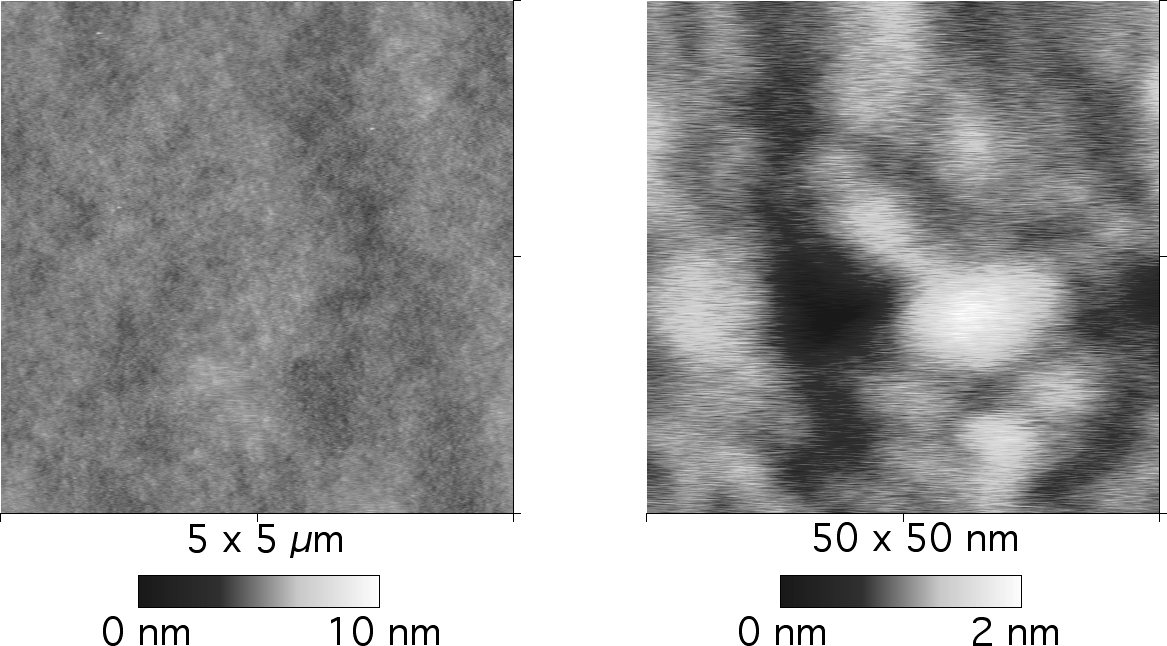
\includegraphics{exp_substrate/CGlas_AFM}
	\begin{minipage}[b]{\linewidth-\tabcolsep-10.3cm}
	\caption[AFM"=Aufnahme eines auf ein Glassubstrat aufgedampften Kohlenstofffilms]{AFM"=Aufnahme eines auf ein Glassubstrat aufgedampften Kohlenstofffilms, dessen Dicke ca.\ \unit[15]{nm} beträgt. (Messung von 26.10.2000, Aufnahmen glc8.000 und glc8.003)}
	\label{fig:afm_c}
	\end{minipage}
\end{figure}

\subsubsection{Verwendung von Kohlenstofffilmen}

\begin{figure}[h!tb]
	\plotlink{c_cooldown}{\includegraphics[width=\smidwidth]{exp_substrate/c_cooldown}}%
	\hfill%
	\begin{minipage}[b]{\linewidth-\tabcolsep-\smidwidth}
		\caption[Verhalten der Transmission während des Abkühlens eines C"=Substrats]{Abkühlen eines Kohlenstoffsubstrats. Die Transmission hat hier ein Maximum von \unit[-50]{dB} (Messung \datalink{2000/mw0012d1/mw0012d1.html}{12/2000 \#1}). Erreichte maximale Güte-/Transmissionwerte bei verschiedenen Messungen: \datalink{2000/mw0010d1/mw0010d1.html}{10/2000 \#1}: 8000 $\unit[-45]{dB}$, \datalink{2000/mw0011d1/mw0011d1.html}{11/2000 \#1}: 2500 $\unit[-42]{dB}$, \datalink{2000/mw0012d1/mw0012d1.html}{12/2000 \#1}: 2000 $\unit[-50]{dB}$, \datalink{2000/mw0012d2/mw0012d2.html}{12/2000 \#2}: 2500 $\unit[-45]{dB}$. Für diesen Messbereich des Zellenthermometers gibt es keine verlässliche Eichung, da die Temperatur hier zwischen \unit[77]{K} und \unit[4.2]{K} liegt. Der Übergangsbereich  bei Sensorwiderständen von $\unit[10]{\Omega}$ bis $\unit[100]{\Omega}$ entspricht jedoch näherungsweise einem Temperaturbereich von \unit[20]{K} bis \unit[10]{K}.\label{fig:c_cooldown}}
	\end{minipage}
\end{figure}

Die so präparieren Kohlenstofffilme wurden erfolgreich als Substrat in den Resonator eingebaut, mit Leitsilber auf beiden Seiten kontaktiert und schon vor und während des Abkühlens konnte ein Transmissionssignal beobachtet werden, dass mit den Messungen mit Siliziumsubstraten vergleichbar ist. Eine erste Messung ist \datalink{2000/mw0011d1/mw0011d1.html}{11/2000 \#1} mit einem \unit[7]{nm} C"=Film mit \unit[5]{mm} Breite, Kaltwiderstand längs ca.\ \unit[8]{M$\Omega$} ; weiterhin wurde in \datalink{2000/mw0012d1/mw0012d1.html}{12/2000 \#1} ein \unit[15]{nm} C"=Film mit \unit[7]{nm} Breite, Kaltwiderstand längs ca.\ \unit[1]{M$\Omega$} untersucht. Leider war es hierbei nicht möglich, Elektronen auf Bulk"=Helium mit einem Kohlenstoff"=Substrat anzusammeln. Die Ursache dafür kann allerdings auch an anderer Stelle im Experiment zu finden sein. Der oben schon angesprochene große Vorteil von dünnen Kohlenstofffilmen als Elektrodenmaterial zeigte sich aber auch schon hier. Selbst bei Raumtemperatur läßt sich das Verhalten der Resonanz des \HR{}s gut beobachten und optimieren.

Falls die erzeugten Kohlenstofffilme zu rau sind, um einen dünnen Heliumfilm darauf mit Elektronen zu beladen, bietet sich noch die Möglichkeit, den Kohlenstofffilm mit einer isolierenden Schicht aus PMMA zu überziehen. Weiterhin ist es auch denkbar, einen Kohlenstofffilm auf die Unterseite eines sehr dünnen isolierenden Substrats aufzubringen, um dann den Heliumfilm auf der Oberseite mit Elektronen zu beladen -- also das Substrat selbst als isolierende Schicht zu verwenden.

Ein großer Vorteil der aufgedampften Kohlenstofffilme ist die Unabhängigkeit von der Leitfähigkeit des verwendeten Substratmaterials -- es können beliebige Isolatoren als Substrate verwendet werden -- und auch die Möglichkeit über die Verwendung von Masken, strukturierte Filme aufzudampfen. Hiermit kann man auf eine einfache Art und Weise z.~B. eine Guard"=Elektrode zur Einschränkung des lateralen Elektronenverlustes (siehe Abschnitt~\ref{ssec:elektronenverlust}) mit auf das Substrat aufbringen.

\subsection{Die Verarbeitung von Silizium"=Substraten}
In den folgenden Abschnitten soll nachvollziehbar dargestellt werden, welche einzelnen Schritte bei der Präparation der verschiedenen Silizium"=Substrate durchgeführt wurden.
\begin{figure}[h!tb]
	\plotlink{si_cooldown}{\includegraphics[width=\smidwidth]{exp_substrate/si_cooldown}}%
	\hfill%
	\begin{minipage}[b]{\linewidth-\tabcolsep-\smidwidth}
		\caption[Verhalten der Transmission während des Abkühlens eines Si"=Substrats]{Verhalten der Transmission und des Substratwiderstandes beim Abkühlen eines Siliziumsubstrats. Die Transmissionskurve verläuft im Vergleich zu einem Kohlenstoffsubstrat in Abbildung~\ref{fig:c_cooldown} sehr steil und die Resonanz wird erst bei Temperaturen unter \unit[20]{K} messbar. (Messung \datalink{2000/mw0204d4/mw0204d4.html}{04/2002 \#4}) Für diesen Messbereich des Zellenthermometers gibt es keine verlässliche Eichung, da die Temperatur hier zwischen \unit[77]{K} und \unit[4.2]{K} liegt. Der Übergangsbereich  bei Sensorwiderständen von $\unit[10]{\Omega}$ bis $\unit[100]{\Omega}$ entspricht jedoch näherungsweise einem Temperaturbereich von \unit[20]{K} bis \unit[10]{K}.\label{fig:si_cooldown}}
	\end{minipage}
\end{figure}

\subsubsection{Reinigungsschritte bei der Verarbeitung}
Alle verwendeten Substrate wurden mit vergleichbaren Prozeduren gereinigt. Bei den mit PMMA zu beschichtenden Substraten wurde diese Reinigung direkt vor dem Aufbringen des PMMA"=Films durchgeführt. Die Silizium- und \SiO/Silizium-Substrate wurden direkt vor dem Einbau in die Messzelle nach der beschriebenen Vorgehensweise gereinigt.
\begin{figure}[h!tbp]
	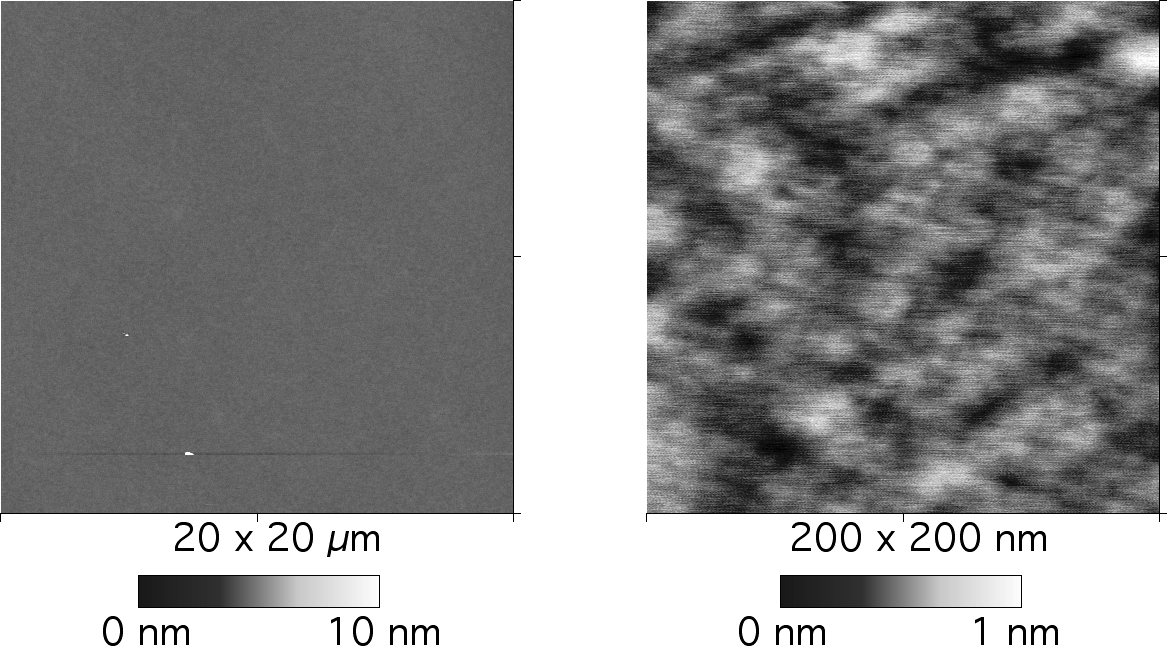
\includegraphics{exp_substrate/SiO2_AFM}
	\begin{minipage}[b]{\linewidth-\tabcolsep-9.9cm}
	\caption[AFM"=Aufnahmen der Oberfläche des \SiO"=Substrats]{AFM"=Aufnahmen der Oberfläche des \SiO"=Substrats, das in den Experimenten verwendet wurde. Auf der rechten Seite ist hier die $z$-Skala im Gegensatz zu den anderen AFM"=Aufnahmen nur \unit[1]{nm}}
	\label{fig:afm_sio2}
	\end{minipage}
\end{figure}

Die Vorräte an Silizium und oxidierten Silizium"=Wafern wurden immer in einer Flow"=Box gelagert, um eine grundlegende Verschmutzung zu vermeiden. Daher wurde auch auf eine nasse Reinigungsmethode verzichtet, wie sie üblicherweise für Substrate verwendet wird. Im Folgenden werden die einzelnen Schritte des Reinigungsprozesses vorgestellt:
\begin{enumerate}
	\item Schneiden des Siliziums in die benötigte Größe in der Flow"=Box. Zu Beginn erfolgt das Anritzen der Schneidelinien mit dem Glasschneider. Danach erfolgt das Brechen des Wafers entlang der Schneidelinien durch vorsichtiges Ausüben von Druck auf den mit der Schneidelinien direkt über einer Kante (z.~B. am Rand eines Geodreiecks) gelagerten Wafers. Dabei wird versucht, eine Berührung der polierten Waferoberfläche, vor allem im Bereich in dem später das 2DES erzeugt werden soll, zu vermeiden. Danach werden die beim Ritzen mit dem Glasschneider und beim Brechen unvermeidbar entstehenden Silizium"=Partikel als erster Reinigungsschritt mit Stickstoffgas aus der Druckflasche abgeblasen.
	\item Reinigung des Substrats mit dem \glqq Snow"=Jet\grqq. Die Oberfläche des Substrats wird vorsichtig mit einem Strahl aus festen Kohlendioxidpartikeln überstrichen. In diesem Schritt werden vorhandene Silizium"=Splitter und andere vorhandene Schmutzpartikel beseitigt, die durch das Abblasen mit Stickstoff nicht entfernt werden konnten.
	\item Eventuell: Weitere Reinigung im Plasmacleaner. Hierbei werden noch vorhandene organische Verunreinigungen entfernt. Für die \SiO"=Substrate ist dieser Schritt wegen der möglichen Erzeugung von Oberflächenladung im Plasma problematisch. Kurze Verweildauern im Plasma im Bereich von \unit[10--30]{s} können jedoch ohne merkbare Verschlechterung der später aufgenommenen Messsignale angewendet werden.
\end{enumerate}

Zur Reduktion von lateralem Elektronenverlust wurde bei manchen Substraten vor dem Einbau eine Isolation der seitlichen Bruchkanten durchgeführt. Weitere Einzelheiten zu dieser Vorgehensweise finden sich im Abschnitt~\ref{ssec:elektronenverlust}.

\subsection{Präparation der PMMA-Filme}
Um Verunreinigungen der Substrate durch Silizium"=Bruchstücke zu vermeiden die beim  Ritzen und Brechen des Siliziumwafers entstehen, wurden diese im Gegensatz zur bisherigen Vorgehensweise bereits vor dem Reinigen und Aufbringen der PMMA"=Isolationsschicht in die im Experiment benötigte Form gebracht. Diese Methode hat darüber hinaus den Vorteil, dass sich auf Grund der langgestreckten Geometrie der Probe beim Aufspinnen des PMMA"=Films am langen Rand der Substratoberfläche ein dickerer PMMA"=Film ausbildet, der das Abfließen der Elektronen in die leitfähige Bruchfläche des Silizium vermindert. Dieser Effekt ist in den Aufnahmen in Abbildung~\ref{fig:substrat_pmma} an der sich aufgrund der Filmdickenänderung anderen Interferenzfärbung des Films deutlich zu sehen.

\begin{figure}[htp!]
	\includegraphics[width=0.6\linewidth]{exp_substrate/substrate68}%
	\hskip -1.5cm%
	\begin{minipage}[b]{0.4\linewidth+1.5cm}
		\caption[Photo des PMMA/Si"=Substrats \#68]{Der Siliziumstreifen von Substrat \#68 mit präpariertem PMMA"=Film. Durch die unterschiedliche Färbung aufgrund der Interferenzen am dünnen Film kann man einen Hinweis auf die Schichdicke des PMMA"=Films erhalten. Zu sehen ist die Erhöhung der PMMA"=Filmdicke am langen Substratrand (Pfeile) und die Spuren ungleichmäßiger Verteilung der Filmdicke aufgrund der länglichen Substratform (Ellipsen). Den Hintergrund bildet Millimeterpapier, um die Größe der Probe abschätzen zu können.}
		\label{fig:substrat_pmma}
	\end{minipage}
\end{figure}

\enlargethispage{-1\baselineskip}
Das vorbereitete Substrat wird auf dem Drehteller der Aufspin"=Anlage fixiert und zur weiteren Reinigung der Oberfläche dort zuerst mit Methanol bedeckt, das nach einigen Sekunden Einwirkungszeit wieder mit maximaler Drehzahl entfernt wird. Danach wird ca.\ \unit[100]{\grmu l}  der PMMA"=Lösung -- mit Konzentrationen im Bereich von 1.25 bis 10 Gewichtsprozent -- mit der Pipette auf das Substrat aufgebracht und mit Drehzahlen von ca.\ \unit[4500]{U/min} mit Beschleunigungszeit 0 wieder entfernt. Nach ca.\ 20 Sekunden andauernder Rotation ist das Lösungsmittel des PMMA ausreichend verdampft und das Substrat kann zur Weiterverarbeitung ausgebaut werden. Um nun noch restliches Lösungsmittel aus dem Substrat zu entfernen und kleinere  
Unregelmäßigkeiten der Oberfläche auszugleichen, wurden die frisch beschichteten Substrate für mindestens zwölf Stunden im Ofen bei ca.\ \unit[60]{°C} im abgepumpten Exsikkator getempert\footnote{Die Lagertemperatur sollte dabei geringer als die Temperatur des Glasübergangs von PMMA von ungefähr \unit[80]{°C} sein.}. Nach dieser Prozedur sind die Substrate bereit für eine Verwendung im Experiment und werden zur weiteren Lagerung im evakuierten Exsikkator belassen.
\begin{figure}[h!tbp]
	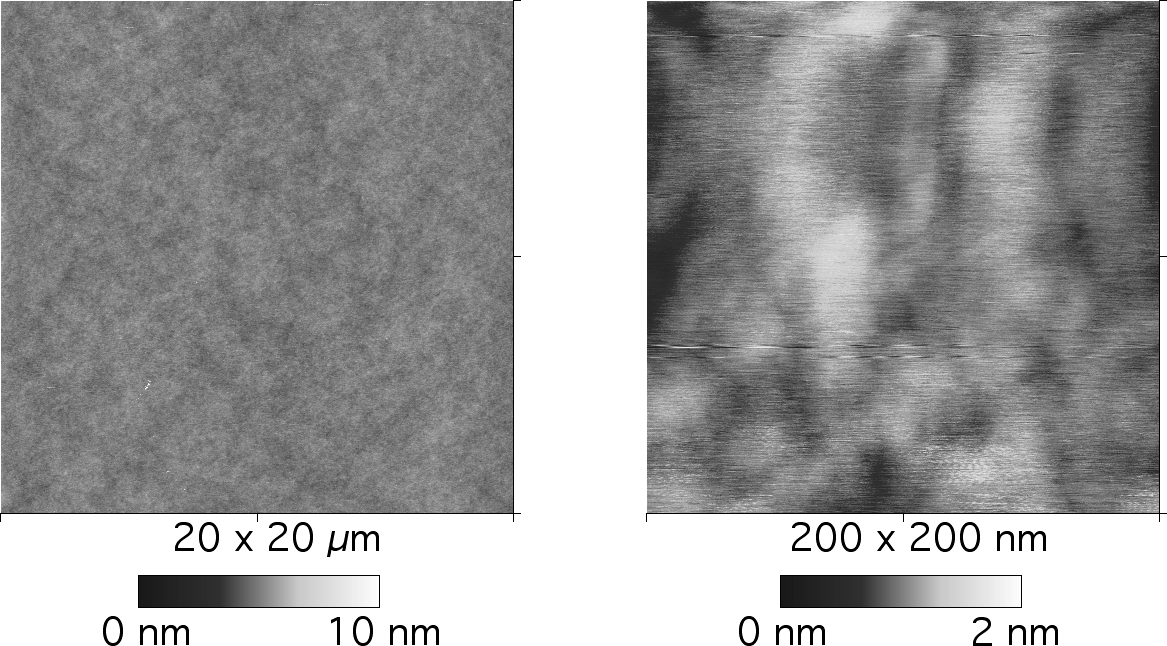
\includegraphics{exp_substrate/PMMA_AFM}
	\begin{minipage}[b]{\linewidth-\tabcolsep-10.3cm}
	\caption[AFM"=Aufnahmen der Oberfläche eines PMMA"=Substrats]{AFM"=Aufnahmen von Substrat \#31, PMMA auf Wacker Si"=Wafer, 10 gew.~\% PMMA gelöst in Essigsäure, Aufgesponnen mit \unitfrac[3000]{U}{min}}
	\label{fig:afm_pmma}
	\end{minipage}
\end{figure}

\subsubsection{Bestimmung der PMMA"=Filmdicke}
\begin{figure}[h!tbp]
	\centerline{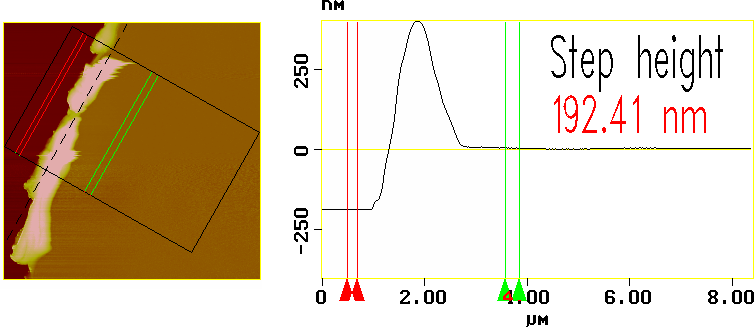
\includegraphics[width=\midwidth]{exp_substrate/sh0109d2}}
	\caption[Bestimmung der PMMA"=Filmdicke]{Bestimmung der Filmdicke des aufgesponnenen PMMA"=Films nach der Verwendung der Substrate. Es wird die Stufenhöhe eines Kratzers im Film mittels einer AFM"=Aufnahme bestimmt. (Substrat \#35. verwendet in Messung \datalink{2001/mw0104d1/mw010d4d1.html}{04/2001 \#1})}
	\label{fig:pmma_thickness}
\end{figure}
Um die PMMA"=Filmdicke zu bestimmen, gibt es verschiedene Möglichkeiten. Zum einen kann man durch den Vergleich zu Substraten mit bekannter PMMA"=Filmdicke aus der durch Interferenzfärbung der Schicht gut die erwartete Größenordnung der Schichtdicke abschätzen. Zum anderen gibt es optische Methoden, wie zum Beispiel ellipsometrische Messungen. Im Gegensatz zu einer solchen zerstörungsfreien Messung mit Ellipsometrie wurde immer die Bestimmung der Tiefe eines in den Film eingeritzen Grabens mit dem AFM durchgeführt.
In Abbildung~\ref{fig:pmma_thickness} ist ein Beispiel für ein Resultat aus dieser Methode zu sehen.
